\section{Multipolar fields for spherical problems}\label{sec:2}

This chapter introduces the multipolar fields as solutions of Maxwell's equations for problems with spherical symmetry. These fields will be expressed in a basis of the so-called multipolar modes. I will provide an overview of two different approaches that lead to a multipolar expansion of the field in different coordinate systems.

In general, we will consider electromagnetic fields in linear, isotropic, and homogeneous media. Such fields are fully described by an electric and magnetic field, \( \mathbf{E} \) and \( \mathbf{H} \), that for the aforementioned conditions need to satisfy the vectorial Helmholtz equation, obtained by the Maxwell equations:
\begin{equation}
    \label{eq:helmholtz}
    \nabla^2\mathbf{E} + k^2\mathbf{E} = 0 \qquad \qquad \nabla^2\mathbf{H} + k^2\mathbf{H} = 0
\end{equation}
where \( k = 2\pi / \lambda \) is the wave number.

This section will demonstrate how the above two equations can be solved by expanding \( \mathbf{E} \) and \( \mathbf{H} \) in multipolar modes, constructed by first solving the scalar wave equation,
\begin{equation}\label{eq:helmholtz_scalar}
    \nabla^2 \psi + k^2 \psi = 0,
\end{equation}
in spherical coordinates by separation of variables, \( \psi(r, \theta, \varphi) = \zeta(r) Y(\theta, \varphi) \).

Inserting this solution in the Helmholtz equation will yield independent ordinary differential equations for the radial and angular part. The radial equation has the spherical Bessel functions, \( j_j(r) \) and \( y_j(r) \) (or any linear combination thereof) as solutions, while the angular equation will be satisfied by the spherical harmonics).

Using the multipolar basis to expand \( \mathbf{E} \) and \( \mathbf{H} \), we may describe \textit{any} electromagnetic field with such components. We will later see that this is a smart choice when describing the scattering process of spherical particles.

\subsection{Approach 1: Spherical polarisation vectors}\label{sec:2_bohren}
One approach to deriving the multipoles is to construct them from the spherical unit vectors, \( \mathbf{\hat{r}}, \boldsymbol{\hat{\theta}} \), and \( \boldsymbol{\hat{\varphi}} \), and the solution of the scalar wave equation, \( \psi \). This approach is taken in \cite{bohren}, which leads to the so-called \textit{magnetic mode} (or transverse electric mode), \( \mathbf{M} = \nabla \times (\mathbf{r} \psi) \), and an \textit{electric mode} (transverse magnetic) as \( \mathbf{N} = \nabla \times \mathbf{M} / k \). Here, \( \mathbf{r} = r \hat{\mathbf{r}} \) is the radial vector.

Using the solutions of the scalar Helmholtz equation, the multipolar modes have the following expressions in the spherical basis and coordinates:
\begin{align*}
\mathbf{M}_{jm_z} &= \frac{m_z}{\sin \theta} P_j^{m_z}(\cos\theta) \zeta_j(kr) e^{im_z \phi} \, \boldsymbol{\hat{\theta}} - \frac{\mathrm{d} P_j^{m_z}(\cos\theta)}{\mathrm{d} \theta} \frac{\zeta_j(kr) e^{im_z \phi}}{\zeta_j(kr)} \, \boldsymbol{\hat{\varphi}} \\
\mathbf{N}_{jm_z} &= j(j + 1) P_j^{m_z}(\cos\theta) \frac{\zeta_j(kr)}{kr} e^{im_z \phi} \, \mathbf{\hat{r}} + \frac{1}{kr} \frac{\mathrm{d} \left[ kr \zeta_j(kr) \right]}{\mathrm{d} (kr)} \frac{\mathrm{d} P_j^{m_z}(\cos\theta)}{\mathrm{d} \theta} e^{im_z \phi} \, \boldsymbol{\hat{\theta}} \\
&\quad + i e^{im_z \phi} \frac{m_z}{\sin \theta} P_j^{m_z}(\cos\theta) \frac{1}{kr} \frac{\mathrm{d} \left[ kr \zeta_j(kr) \right]}{\mathrm{d} (kr)} \, \boldsymbol{\hat{\varphi}}
\end{align*}
\( j \in \mathbb{N}_0 \) and \( m_z \in [-j, j] \) are indices appearing in the differential equations.

Any incident EM field can then be expanded in this basis by proving that the modes are orthogonal for all \( j, m_z \) and ensuring that the sum converges and is normalised by appropriate choice of coefficients, \( g^{(m)}_{jm_z} \) and \( g^{(e)}_{jm_z} \) \cite{bohren}:
\begin{equation}\label{eq:E_i_expansion}
    \mathbf{E}_i = \sum_{j=0}^\infty \sum_{m_z=-j}^j g_{jm_z}^{(m)} \mathbf{M}_{jm_z} + g_{jm_z}^{(e)} \mathbf{N}_{jm_z}.
\end{equation}

As an example to be compared with the other approach, I will present the plane-wave expansion in this basis, which in the Cartesian basis has the simple expression for a plane wave propagating along the \( z \)-axis and polarised along the \( x \)-axis:
\begin{equation}\label{eq:PW_cart}
     \mathbf{E}_i = E_0 e^{ikr \cos\theta} \mathrm{\mathbf{e}}_x
\end{equation}
It can be shown that all coefficients except \( g^{(m)}_{j,1} \) and \( g^{(e)}_{j,1} \) vanish. Following the notation in \cite{bohren}, each mode can also be separated in an even and odd component, e.g., \( \mathbf{M}_{ejm_z} \) and \( \mathbf{M}_{ojm_z} \). This yields the simplified expansion of the plane wave:
\begin{equation}\label{eq:PW_sph}
    \mathbf{E}_i = E_0 \sum_{j=1}^\infty i^j \frac{2j+1}{j(j+1)} (\mathbf{M}_{oj1} - i \mathbf{N}_{ej1})
\end{equation}

\subsection{Approach 2: Angular momentum method}\label{2_rose}
Another way of defining the multipoles is provided by M.E. Rose in \cite{rose}. This section follows his notation. In this approach, the multipoles are demanded to be eigenfunctions of the z-component of the angular momentum operator, \( \mathbf{J} = \mathbf{L} + \mathbf{S} \), and its square, \( \mathbf{J}^2 \). The eigenfunctions of the orbital angular momentum operators are the spherical harmonics, \( Y_l^{m_z} \),
\begin{equation}\label{eq.sphharm}
    L_z Y_l^{m_z} = m_z Y_l^{m_z} \qquad \mathbf{L}^2 Y_l^{m_z} = l(l+1) Y_l^{m_z},
\end{equation}
and the spin eigenfunctions are the normalized spherical basis vectors:
\begin{equation}\label{eq:S_ev}
    \boldsymbol{\xi}_1 = -\frac{1}{\sqrt{2}} (\mathbf{\hat{x}} + i \mathbf{\hat{y}}) \qquad
    \boldsymbol{\xi}_0 = \mathbf{\hat{z}} \qquad
    \boldsymbol{\xi}_{-1} = \frac{1}{\sqrt{2}} (\mathbf{\hat{x}} - i \mathbf{\hat{y}}),
\end{equation}
that satisfy the eigenvalue equation \( \mathbf{S} \boldsymbol{\xi}_{\mu} = \mu \mathbf{S} \quad \mu = 1, 0, -1 \). These polarisation vectors correspond to left, \( z \), and right circularly polarised light respectively.

Finding eigenfunctions of \( J_z \) requires finding common eigenfunctions of \( L_z \) and \( S_z \), which is done with the Clebsch-Gordan coefficients:
\begin{equation}
    \mathbf{T}_{jlm_z} = \sum_{\mu} C(l 1 j; m_z - \mu, \mu) Y_{l}^{m_z - \mu}(\theta, \varphi) \boldsymbol{\xi}_{\mu}
\end{equation}
These are called vector spherical harmonics (VSHs). The sum over \( \mu \) gives the three polarisation components, adding up to one value of \( m_z \).

From the VSHs, the electric and magnetic multipoles can be derived by imposing rules for addition of angular momenta and parity considerations \cite{comparison}, that simplify the VSHs to those with \( l = j, j+1 \), or \( j-1 \). 
Then, leaving only the \( l \) index, the multipoles are written as the product of the spatial and angular components,
\begin{align*}
    \text{Magnetic:}\quad & \mathbf{A}^{(m)}_{lm_z} = C_l^{(m)} \zeta_l(kr) \mathbf{T}_{llm_z}(\theta, \varphi) \\
    \text{Electric:}\quad & \mathbf{A}^{(e)}_{lm_z} = C_{l+1}^{(e)} \zeta_{l+1}(kr) \mathbf{T}_{l,l+1,m_z}(\theta, \varphi) + C_{l-1}^{(e)} \zeta_{l-1}(kr) \mathbf{T}_{l,l-1,m_z}(\theta, \varphi),
\end{align*}
where the coefficients represent normalisation (or gauge) constants.

In this basis with these VSHs, one can also expand a circularly polarised plane wave propagating in \( z \) as:
\begin{equation}\label{eq:rosePW}
    \mathbf{E}_{pw} = ik \mathbf{A}_{pw} = ik \sqrt{2\pi} \sum_{l=1}^{\infty} i^l \sqrt{2l+1} ( \mathbf{A}_{lp}^{(m)} + i p \mathbf{A}_{lp}^{(e)} ),
\end{equation}
As in plane wave expansion, this expression also only sums over the index \( j \), keeping a fixed value of \( m \) (here \( p \), representing the left or right circular polarisation). The electric and magnetic multipole are again separated by a phase of \( i \).

\subsection{Limits}
As mentioned before, any linear combination of the spherical Bessel functions of the first and second kind (also referred to as the spherical Bessel, \( j_j(kr) \), and Neumann, \( y_j(kr) \), functions) satisfy the radial part of the wave equation. However, for \( r \to 0 \), only \( j_j(kr) \) is regular, while \( y_j(kr) \) goes to \( -\infty \). At \( r \to \infty \), both functions are oscillating and thus physical. This means that in the expression for the multipoles, \( \zeta_j(kr) = j_j(kr) \) if its domain spans all space. This is, for example, not the case when working with multipoles in a scattering problem. Here, the spherical Bessel function will be used inside the scatterer, while the Hankel function, \( h_j(kr) = j_j(kr) + i y_j(kr) \), is used outside.

\subsection{Visualisation}
To get an idea of the nature of the multipolar fields, I have plotted two instances of them in the figures below, an electric and a magnetic - both of which have the wavelength \( \lambda = 0.632\ \mathrm{\upmu m} \). The plots show projections of the intensity (norm squared of the three polarisations) onto an XY plane at \( z = 0 \) as well as an XZ plane at \( y = 0 \). The XY plane would therefore be a horizontal slice through the middle of the XZ plane.

In addition, they are divided into the three circular polarization components. Since most readers are more familiar with the scattering multipoles than the internal, the plots use the Hankel function, blocking a central region of radius \( R = 0.25\ \mathrm{\upmu m} \) where it diverges. 
In the top tow of the figure, a magnetic quadrupole (order \( l = 2 \)) is shown with \( m_z = 0 \), i.e., no angular momentum along the \( z \)-axis. 
The magnetic quadrupole has negligible intensity in \( z = 0 \) (notice the low magnitude of the colour scale in the XY slices). Instead, the vast majority of its intensity is concentrated in four 'lobes' visible in the XZ planes (giving the quadrupole name meaning) in the left and right circular polarisation.

\begin{figure}
    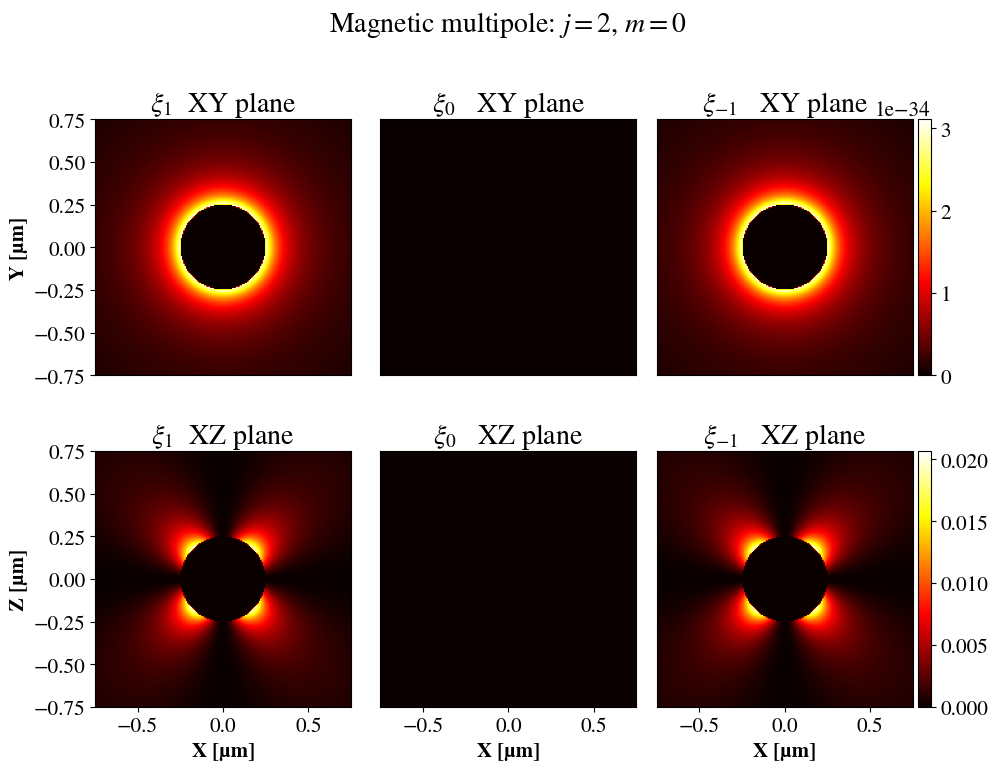
\includegraphics[trim={0 0cm 0 2cm},clip,width=0.8\textwidth]{Figures/mpolej2m0.png}
    \caption{Magnetic multipole with \( l = 2 \) and \( m_z = 0 \). Each row is plotted on its own colour scale.}
    \label{fig:mpole}
\end{figure}

\begin{figure}
    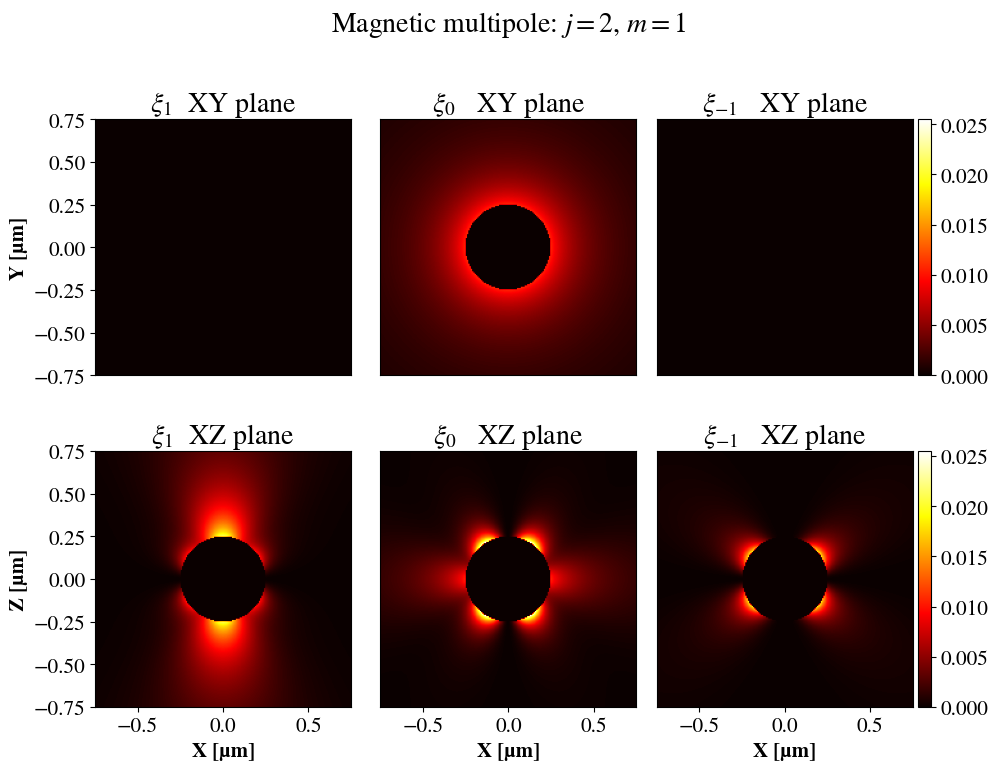
\includegraphics[trim={0 0cm 0 2cm},clip,width=0.8\textwidth]{Figures/epolej2m1.png}
    \caption{Electric multipole with \( l = 2 \) and \( m_z = 1 \). All plots are shown on the same colour scale.}
    \label{fig:epole}
\end{figure}

An electric quadrupole, this time with a non-zero value of \( m_z \), is shown in the bottom row. Here, \( \xi_{-1} \), the right circular polarization, also has four spots of high intensity in the XZ-plane. A larger distribution of intensity is also visible in the XZ plane of the left circular polarisation. Both of these again have negligible intensities in the XY plane at \( z = 0 \).

The \( \xi_0 \) polarisation component has a symmetric, and significantly higher intensity distribution in the XY-plane at \( z = 0 \). In the XZ plane, it has four distinct spots and two broader lobes along the \( x \)-axis.